\documentclass[3p]{elsarticle}
\usepackage{mathpazo,amsmath,amsfonts,amssymb,siunitx,tikz}
\usetikzlibrary{decorations.pathmorphing}
\bibliographystyle{elsarticle-num-names}
\newcommand*{\mT}{\mathrm{T}}
\newcommand*{\figref}[1]{Fig.~\ref{#1}}
\ead{lei.zhang@pg.canterbury.ac.nz}
\begin{document}
\section{Definition of DoFs}
There are two nodes for a typical MVLE model. Due to both boundary beams are simplified to rigid bars, there are six degrees of freedom (DoFs) in each element: one rotational and two translational for each node, as illustrated in \figref{MVLEMFORMULATION}.
\begin{figure}[ht]
\centering\footnotesize
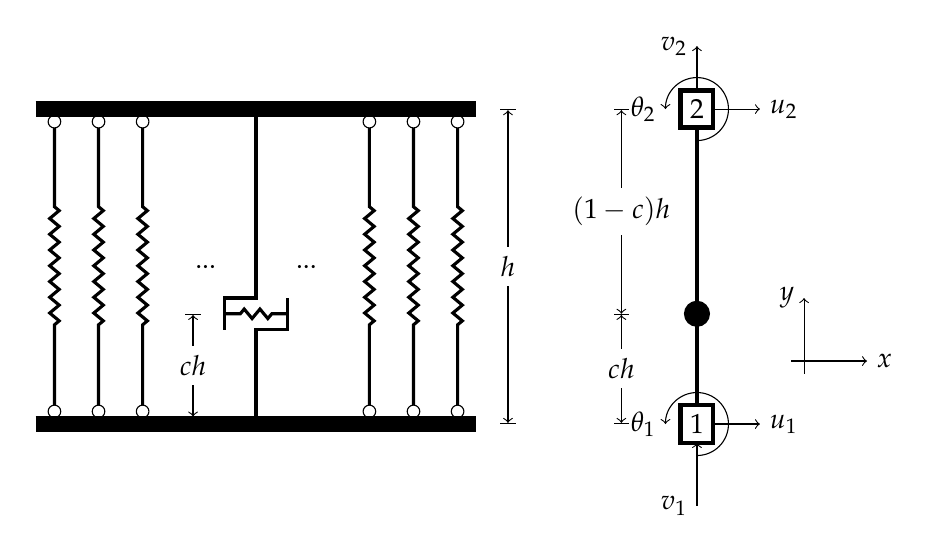
\begin{tikzpicture}[x=1mm,y=1mm,scale=.8]
\def\a{25}\def\b{35}
\draw[line width=.4mm,decorate,decoration={zigzag,pre length=2mm,post length=2mm,amplitude=.6mm,segment length=2mm}](-5,-7.5)--++(10,0);
\foreach\x in{-\b+3,-\b+10,-\b+17,\b-17,\b-10,\b-3}{
\draw[line width=.4mm,decorate,decoration={zigzag,pre length=10mm,post length=10mm,amplitude=.6mm,segment length=2mm}](\x,\a-3)--(\x,-\a+3);
\foreach\d in{-\a+2,\a-2}\draw(\x,\d)circle[radius=1mm];};
\draw[line width=2mm]
	(-\b,\a)--(\b,\a)
	(-\b,-\a)--(\b,-\a);
\draw[line width=.4mm]
	(0,\a)|-(-5,-5)--++(0,-5)
	(5,-5)|-(0,-10)--(0,-\a);
\draw
	(-8,0)node{...}
	(8,0)node{...};
\draw[|<->|](-10,-\a+1)--(-10,-7.5)node[fill=white,midway]{$ch$};
\draw[|<->|](\b+5,-\a)--(\b+5,\a)node[fill=white,midway]{$h$};
\begin{scope}[xshift=70mm]
\draw[->](15,-15)--++(12,0)node[anchor=west]{$x$};
\draw[->](17,-17)--++(0,12)node[anchor=east]{$y$};
\draw[->](0,-\a)--++(10,0)node[anchor=west]{$u_1$};
\draw[->](0,\a)--++(10,0)node[anchor=west]{$u_2$};
\draw[<-](0,-\a-3)--++(0,-10)node[anchor=east]{$v_1$};
\draw[->](0,\a)--++(0,10)node[anchor=east]{$v_2$};
\draw[->](0,-\a-5)arc(-90:180:5)node[anchor=east]{$\theta_1$};
\draw[->](0,\a-5)arc(-90:180:5)node[anchor=east]{$\theta_2$};
\draw[line width=.6mm]
	(0,-\a)node[draw,fill=white]{$1$}--
	(0,-7.5)node[circle,fill=black]{}--
	(0,\a)node[draw,fill=white]{$2$};
\draw[|<->|](-12,-\a)--(-12,-7.5)node[fill=white,midway]{$ch$};
\draw[|<->](-12,\a)--(-12,-7.5)node[fill=white,midway]{$(1-c)h$};
\end{scope}
\end{tikzpicture}
\caption{Definition of DoFs of the MVLE model.}\label{MVLEMFORMULATION}
\end{figure}
% Final.

The displacement vector can be then expressed as
\begin{gather}
\mathbold{a}=\left[\begin{array}{cc}
	\mathbold{a}_1 & \mathbold{a}_2
\end{array}\right]^\mT=
\left[\begin{array}{cccccc}
	u_1 & v_1 & \theta_1 & u_2 & v_2 & \theta_2
\end{array}\right]^\mT.
\end{gather}

The force vector can be expressed as
\begin{gather}
\mathbold{P}=\left[\begin{array}{cc}
	\mathbold{P}_1 & \mathbold{P}_2
\end{array}\right]^\mT=
\left[\begin{array}{cccccc}
	F_1 & V_1 & M_1 & F_2 & V_2 & M_2
\end{array}\right]^\mT.
\end{gather}
\section{Stiffness Matrix Formation}
The element stiffness matrix relates displacement vector with force vector.
\begin{equation}\label{A21}
\mathbf{K}\mathbold{a}=\mathbold{P}.
\end{equation}
The stiffness matrix $\mathbf{K}$ can be easily formed according to virtual work principle (apply unit displacement on every individual DoFs and solve the equilibrium equation).
\begin{gather}
\mathbf{K}=\left[\begin{array}{cccccc}
	k_H &      0       &          -chk_H          & -k_H  &       0       &          (c-1)hk_H           \\
	    &  \sum{}k_i   &       \sum{}k_ix_i       &   0   &  -\sum{}k_i   &        -\sum{}k_ix_i         \\
	    &              & c^2h^2k_H+\sum{}k_ix_i^2 & chk_H & -\sum{}k_ix_i & c(1-c)h^2k_H-\sum{}k_ix_i^2  \\
	    &              &                          &  k_H  &       0       &          (1-c)hk_H           \\
	    & \text{Symm.} &                          &       &   \sum{}k_i   &         \sum{}k_ix_i         \\
	    &              &                          &       &               & (1-c)^2h^2k_H+\sum{}k_ix_i^2
\end{array}\right],\label{MVLEMK}
\end{gather}
where $k_H$ is the stiffness of lateral shear spring, $k_i$ is the stiffness of $i^{\mathrm{th}}$ vertical spring and $x_i$ is the corresponding distance from the central axis. Note that for a more concise expression, the summation notation $\sum\limits_{i=1}^{n}$ is simplified to $\sum$.

The matrix can be further decomposed as
\begin{gather*}
\mathbf{K}=\mathbf{K}^V+\mathbf{K}^H,\\
\mathbf{K}^V=\left[\begin{array}{cc}
	\mathbf{K}^V_{11} & \mathbf{K}^V_{12} \\[2mm]
	\mathbf{K}^V_{21} & \mathbf{K}^V_{22}
\end{array}\right],\quad
\mathbf{K}^V_{11}=\mathbf{K}^V_{22}=-\mathbf{K}^V_{12}=-\mathbf{K}^V_{21}=\left[\begin{array}{ccc}
	0 &      0       &       0        \\[2mm]
	0 &  \sum{}k_i   &  \sum{}k_ix_i  \\[2mm]
	0 & \sum{}k_ix_i & \sum{}k_ix_i^2
\end{array}\right],\\
\mathbf{K}^H=k_H\left[\begin{array}{cccccc}
	1 &      0       &  -ch   & -1 & 0 &   (c-1)h   \\
	  &      0       &   0    & 0  & 0 &     0      \\
	  &              & c^2h^2 & ch & 0 & c(1-c)h^2  \\
	  &              &        & 1  & 0 &   (1-c)h   \\
	  & \text{Symm.} &        &    & 0 &     0      \\
	  &              &        &    &   & (1-c)^2h^2
\end{array}\right].
\end{gather*}

Apparently, it can be seen that the flexure response and shear response are uncoupled as $\mathbf{K}^H$ controls the shear behaviour while $\mathbf{K}^V$ controls the flexure behaviour of the wall. The stiffness matrix $\mathbf{K}$ can also be deduced by a transformation method, though such a method is slightly more complicated.
\begin{gather*}
\mathbf{K}=\mathbold{b}^\mT\mathbf{K}_\text{sub}\mathbold{b},\\
\mathbold{b}=\left[\begin{array}{cccccc}
	 0   & -1 & 0 &  0  & 1 & 0 \\
	-1/h & 0  & 1 & 1/h & 0 & 0 \\
	-1/h & 0  & 0 & 1/h & 0 & 1
\end{array}\right],\\
\mathbf{K}_\text{sub}=
\left[\begin{array}{ccc}
	 \sum{}k_i   &      -\sum{}k_ix_i       &         \sum{}k_ix_i         \\[2mm]
	             & c^2h^2k_H+\sum{}k_ix_i^2 & c(1-c)h^2k_H-\sum{}k_ix_i^2  \\[2mm]
	\text{Symm.} &                          & (1-c)^2h^2k_H+\sum{}k_ix_i^2
\end{array}\right].
\end{gather*}

As eventually the uni-axial constitutive/hysteresis model is adopted for the calculation, to find $k_i$ and $k_H$, the displacement for every individual spring should be found from element displacement vector $a$.
\begin{gather}
\Delta{}l=\mathbold{ca},\label{A22}\\
\mathbold{c}=\left[\begin{array}{cccccc}
	0 & -1 & -x_i & 0 & 1 & x_i
\end{array}\right],\qquad\text{for the $i^{\mathrm{th}}$ vertical spring},\\
\mathbold{c}=\left[\begin{array}{cccccc}
	1 & 0 & -ch & -1 & 0 & (c-1)h
\end{array}\right],\qquad\text{for the shear spring}.
\end{gather}

Then the spring forces can be found according to the Hooke's law
\begin{gather}
f_{i(H)}=k_{i(H)}\Delta{}l_{i(H)}=\dfrac{E_{i(H)}A_{i(H)}}{L_i}\Delta{}l_{i(H)}.\label{A23}
\end{gather}
According to force equilibrium, the force vector $\mathbold{P}$ can be assembled if the force components $f_{i(H)}$ are known.
\begin{gather}
\mathbold{P}=\left[\begin{array}{cccccc}
	f_H & -\sum{}f_i & -chf_H-\sum{}f_ix_i & -f_H & \sum{}f_i & (c-1)hf_H+\sum{}f_ix_i
\end{array}\right]^\mT.\label{A24}
\end{gather}
\end{document}
